\newpage
\section{Material und Methoden}
\label{sec:durchführung}
%Rahmenbedinungen der Untersuchung
%Auswahl, Einschränkungen und Begründungen
%Erhebungs-, Mess- und Auswertungsverfahren
%Womit und wie haben Sie untersucht ?
\subsection{Allgemein heuristisches Entscheidungsverfahren}
Da es sich diese Bachelorarbeit mit der Findung einer Lösung für eine Problemstellung beschäftigt, wird sich in diesem Abschnitt der Lehre der Heuristik zugewandt. Allgemein beschäftigt sich diese Wissenschaft mit Verfahren um Probleme zu lösen. Im Vordergrund stehen hierbei methodische Anleitungen, Anweisungen und Denkalgorithmen zu schaffen, welche zur Gewinnung neuer Erkenntnisse führen. \cite{Duden.10.02.2022} \linebreak Eine Kategorie dieser Verfahren sind allgemein heuristische Entscheidungsverfahren. Das Wort "`allgemein"' bedeutet in diesem Fall, dass die Methodik des Entscheidungsverfahrens nicht für ein spezielles Entscheidungsproblem konzipiert ist, sondern durchaus für verschiedenste Entscheidungsprobleme nutzbar ist. 
Möglichkeiten, die sich aus der Anwendung eines allgemein heuristischen Verfahrens ergeben sind, dass sie:
\begin{itemize}
	\item zur Lösung beliebiger Entscheidungsprobleme geeignet sind,
	\item die Zielorientierung erhöht wird und damit Fehlentscheidungen vermieden werden und
	\item die Trennung von Faktenwissen und persönlicher Bewertung die Entscheidungsqualität erhöht.
\end{itemize}
Jedoch ergeben sich mit diesen Möglichkeiten auch Grenzen wie zum Beispiel, dass:
\begin{itemize}
	\item allgemein heuristische Entscheidungsverfahren weniger effektiv und effizient sind als ein existierendes spezielles Entscheidungsverfahren,
	\item die Vermeidung von Fehlentscheidungen nicht garantiert werden kann und
	\item mangelndes Fachwissen dadurch nicht kompensiert wird.
\end{itemize}

\subsubsection{Entscheidungsverfahren nach \textsc{Grüning} und \textsc{Kühn}}

Im allgemein heuristischen Entscheidungsverfahren nach \textsc{Grüning} und \textsc{Kühn} beschreiben die Autoren auf welcher Grundlage die Entwicklung ihres Verfahrens beruht. Diese umfasst unter anderem heuristische Prinzipien, Entscheidungsmaximen, Erfahrungen der Autoren als Berater für komplexe Entscheidungssituationen, Erfahrung aus der Entwicklung spezieller heuristischer Entscheidungsverfahren, sowie existierenden allgemein heuristischen Entscheidungsverfahren von anderen Autoren. Mehr dazu, sowie die Beschreibung der Arten von Entscheidungsproblemen findet sich in \cite{Grunig.2013}. Das Verfahren von \textsc{Grüning} und \textsc{Kühn} umfasst dabei sieben Schritte, welche über Schrittsequenzen miteinander verknüpft werden (siehe Abbildung \ref{fig:ahev}).  

\begin{figure}[h!]
	\centering
	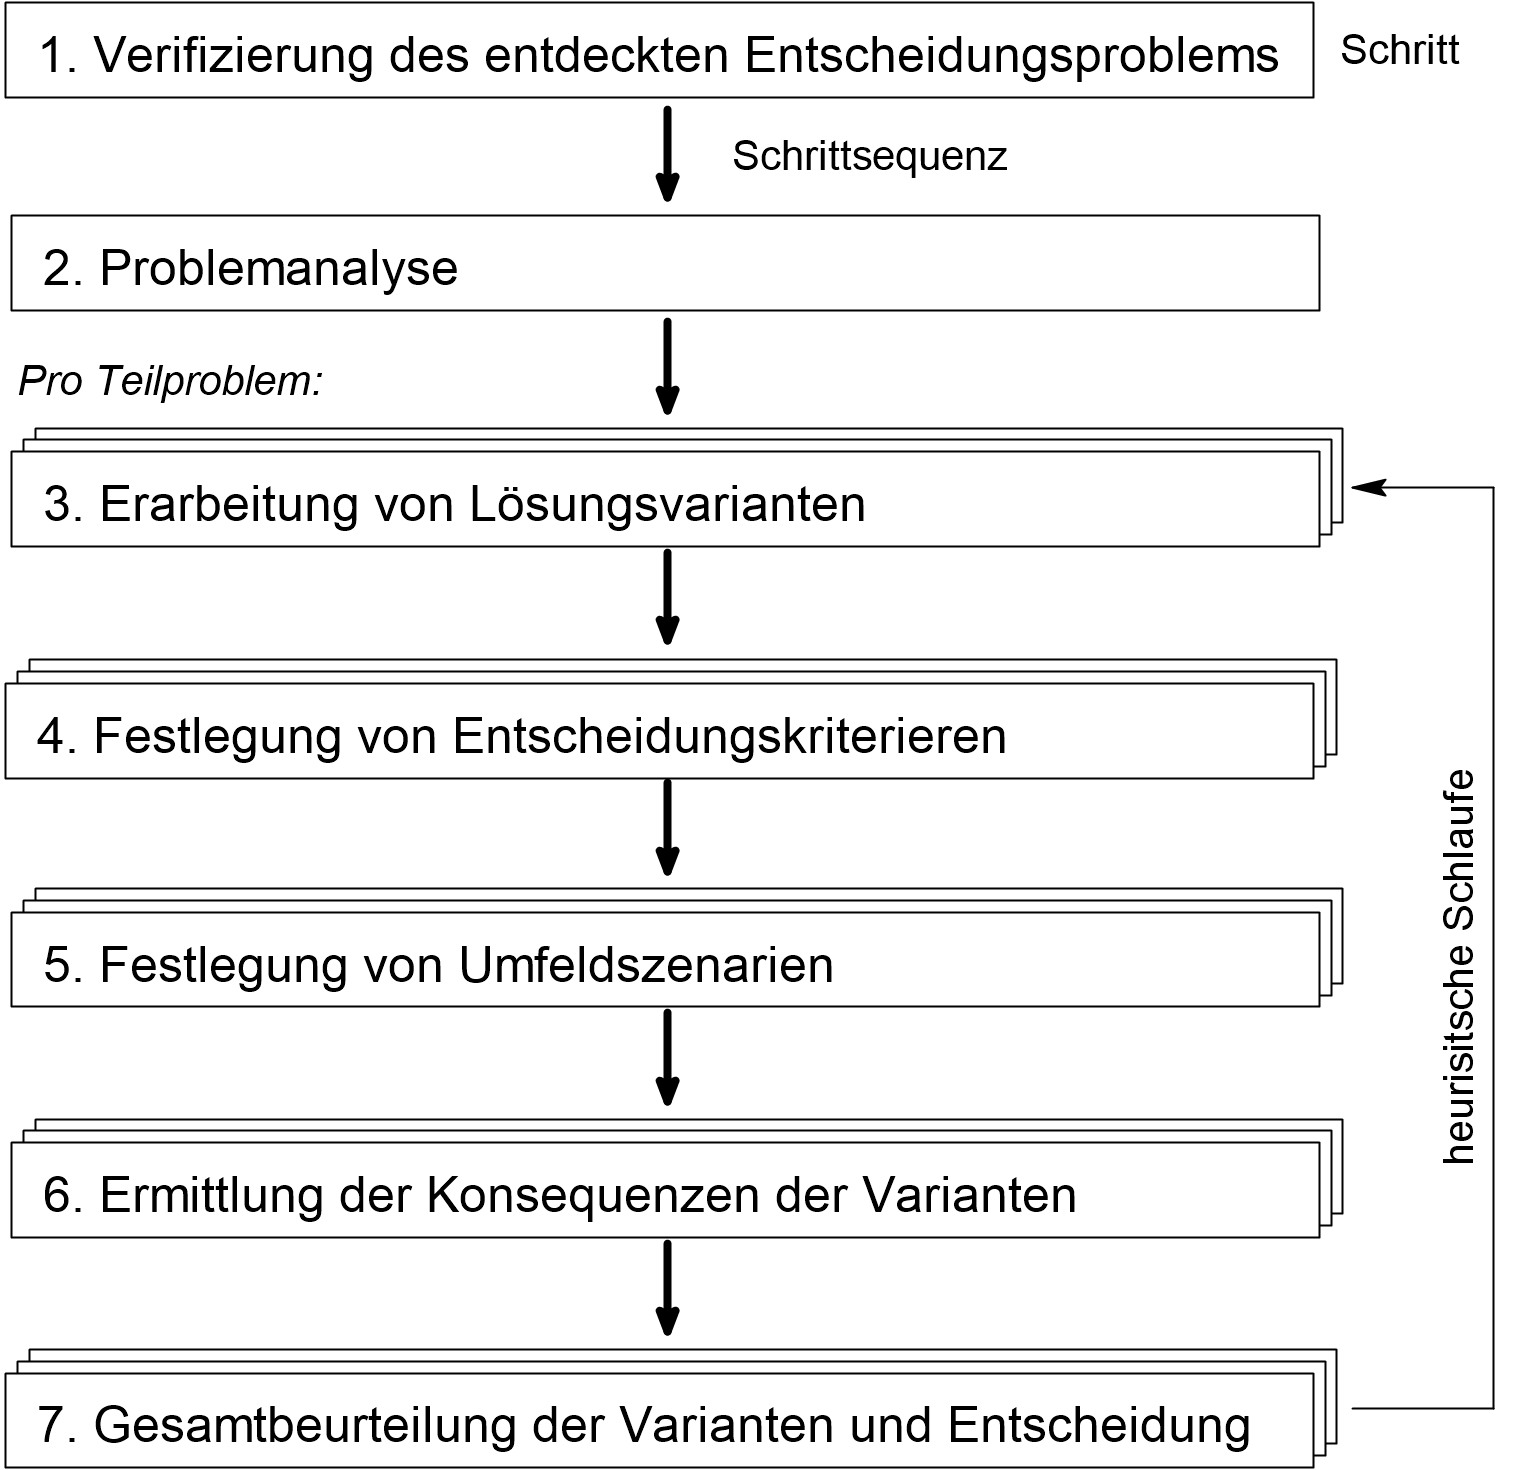
\includegraphics[width=0.5\textwidth]{img/heuristik}
	\caption{Allgemein heuristisches Entscheidungsverfahren, erstellt nach \cite{Grunig.2013}}
	\label{fig:ahev}
\end{figure}
\FloatBarrier

Werden in der Problemanalyse mehrere Teilprobleme festgestellt sind die Schritte\,3 bis 7 für jedes Einzelproblem zu durchlaufen. Die Rückführung, die durch diese Entscheidungsprozesse entsteht wird "`heuristische Schlaufe"' genannt und ist mit dem am häufigsten auftretenden Vertreter in der Entscheidungsfindung in Abbildung \ref{fig:ahev} darstellt. Solche Rückführungen der Entscheidungsschritte können in allen Prozessschritten vorkommen und somit kann es in jeder Teilaktivität zu solch heuristischen Schlaufen kommen. So kann es passieren, dass die Entscheidungskriterien unter Schritt 4 angepasst werden müssen, während bereits in Schritt 6 die Konsequenzen der Lösungsvarianten bestimmt werden. \cite{Grunig.2013} Um das Verfahren anwenden und besser verstehen zu können, werden die einzelnen Schritte des Entscheidungsverfahrens kurzerhand näher erläutert. 
\vspace*{-2.5mm}
\paragraph{Schritt 1: Verifizierung des entdeckten Entscheidungsproblems} In diesem Schritt ist zu prüfen ob die Bearbeitung des Entscheidungsproblems lohnenswert ist und in wie fern sich Soll- und Ist-Zustand voneinander abweichen und auf verlässliche Informationen zurückführen lassen. Lässt sich die Bearbeitung des Problems als lohnenswert und die Beschreibung des Soll- und des Ist-Zustandes auf valide Informationen zurückzuführen ist, gilt das Problem als verifiziert. Je nach Wichtigkeit und Dringlichkeit wird dann festgelegt wer und in welchem Zeitraum an dem Entscheidungsproblem gearbeitet werden soll. Ist keine Aussage zur Wichtigkeit und Dringlichkeit möglich wird von beiden der Worst-Case angenommen.
\vspace*{-2.5mm}
\paragraph{Schritt 2: Problemanalyse} In diesem Schritt wird die Problemstellung abgegrenzt und strukturiert. Im Zuge dieser Analyse erfolgen dann Recherchen und Ermittlungen von relevanten Informationen, um die Problemursachen festzustellen und das Problem in mehrere Teilprobleme zu zerlegen. Danach wird festgelegt welche dieser einzelnen Probleme parallel oder nacheinander bearbeitet werden können. Diese Struktur ist maßgeblich für das Vorgehen in den folgenden Schritten.\\

Die folgenden Schritte 3 bis 7 werden mit jedem Teilproblem einzeln durchgeführt und es kann gegebenenfalls zu heuristischen Schlaufen innerhalb dieser Bearbeitungsschritte kommen. Je nach vorgegebener Struktur unter Schritt 2 kann die Bearbeitung dieser Teilprobleme unterschiedlich angegangen werden.
\vspace*{-2.5mm}
\paragraph{Schritt 3: Erarbeitung von Lösungsvarianten} In diesem Schritt des Entscheidungsverfahrens werden mindestens zwei oder mehr Lösungsvarianten für das Teilproblem erarbeitet. Um den weiteren Bewertungsprozess des Entscheidungsverfahrens rechtfertigen zu können, ist bei der Erarbeitung der Varianten zu beachten, dass sich diese in wesentlichen Merkmalen und nicht nur in Details unterscheiden. 
\vspace*{-2.5mm}
\paragraph{Schritt 4: Festlegung von Entscheidungskriterien} Sind die Lösungsvarianten bestimmt, gilt es sich als nächstes die Entscheidungskriterien festzulegen anhand derer die Varianten evaluiert werden sollen. Die Beschreibung dieser Kriterien besticht dabei durch konkret definierte Maßstäbe anhand derer eine Einschätzung erfolgen kann.
\vspace*{-2.5mm}
\paragraph{Schritt 5: Festlegung von Umfeldszenarien} Dieser optionale Schritt des Entscheidungsprozesses fordert den Aktor der Entscheidung dazu auf, falls nötig, verschiedene Szenarien des Umfeldes zu beschreiben und Eintrittswahrscheinlichkeiten dafür zu definieren. In der Risiko- und Gefahrenanalysen nach dem HAZOP-Verfahren findet eine solche Beurteilung des Umfeldes beispielsweise statt. \todo{Münch nachfragen ob diese Riskotabelle nur für HAZOP galt}
\vspace*{-2.5mm}
\paragraph{Schritt 6: Ermittlung der Konsequenzen der Varianten:} Die zuvor überlegten Entscheidungskriterien und die optionalen Umweltszenarios werden mit den erarbeiteten Lösungsvorschlägen in einer Entscheidungsmatrix zusammengefasst und die sich daraus ergebenen Konsequenzwerte eingetragen. Die Konsequenzwerte werden hierbei durch eingehende Recherchen und dem Wissen und der Erfahrung des Aktors bestimmt und können daher auch einer gewissen Subjektivität unterliegen.
\vspace*{-2.5mm}
\paragraph{Schritt 7: Gesamtbeurteilung der Varianten und Entscheidung} Im letzten Schritt werden die einzelnen Lösungsvarianten in ihrer Gesamtheit beurteilt. Dafür werden irrelevante Varianten eliminiert und danach bestimmt ob für die Wahl der Lösungsvariante ein analytisches oder summarisches Vorgehen bevorzugt wird. Dies entscheidet sich dadurch ob lediglich ein (Einwertigkeit) oder mehrere voneinander unabhängige Entscheidungskriterien (Mehrwertigkeit) die Alternativen unterscheiden und ob es unkontrollierbare Situationen gibt, die für die Variantenwahl entscheidend sind. Im Normalfall kann bei komplexen Problem davon ausgegangen werden, dass diese mehrwertig sind und/oder eine gewisse Unsicherheit oder Ungewissheit der Situation in sich tragen. Laut \cite{Grunig.2013} wird daher ein analytisches Vorgehen bevorzugt bei der Hilfswerte gebildet und verrechnet werden können. Alternativ dazu können sich bei einwertigen und/oder sicheren Entscheidungen auch summarisches Vorgehen eignen, da diese durch Abwägung der Vor- und Nachteile der Varianten weniger komplex und besser interpretierbar sind. 
In der Literatur sind für die jeweiligen Vorgehensweisen verschiedene Methoden, sogenannte Entscheidungsmaximen beschrieben, welche die Überwindung von Mehrwertig, Unsicherheit oder Ungewissheit möglich machen. Eine Möglichkeit der Überwindung der Mehrwertigkeit und der Unsicherheit ist zum Beispiel die auf \textsc{Bernoulli} zurückgehende Maxime des Nutzenerwartungswertes.\linebreak
Ist die Bestimmung der Varianten für die einzelnen Teilprobleme nach analytischen oder summarischen Vorgehen erfolgt, können infolgedessen die vorgeschlagenen Varianten der Teilprobleme mit einander abgestimmt werden. Bildet sich dabei keine heuristische Schleife fällt die Entscheidung über die zu realisierende Variante.

\subsubsection{Nutzenwertmaxime}
Für das analytische Vorgehen bei der Gesamtbeurteilung der Varianten kann die Nutzenwertmaxime zur Überwindung von Mehrwertigkeit genutzt werden. Sie unterscheidet sich von der Maxime des Nutzenerwartungswertes nach \textsc{Bernoulli} durch die fehlende Einbeziehung des Erwartungswertes und überwindet somit auch keine Unsicherheiten. Das muss jedoch bei sicheren Situationen der Entscheidung keinen Nachteil mit sich bringen. Die Entscheidung einer Variante mittels Nutzenwertmaxime umfasst vier Teilaufgaben: 
\vspace*{-2.5mm}
\paragraph{Schritt 1: Umrechnung nicht-numerischer Konsequenzwerte}	\, \\
Nicht-numerische Konsequnzwerte sind anhand einer definierten Skala in Zahlenwerte umzurechnen.
\vspace*{-2.5mm}
\paragraph{Schritt 2: Umrechnung der Konsequenzwerte in Nutzenwerte} \, \\ 
Für jedes Entscheidungskriterium hat die Summe an Nutzwerten der Variante "`1"' zu betragen. Die Nutzwerte der Varianten sind dabei so zu bestimmen, dass die Nutzenwerte zwischen $0$ und 1 liegen und das die günstigste Konsequenz den höchsten Nutzenwert besitzt.
\vspace*{-2.5mm}
\paragraph{Schritt 3: Gewichtung der Entscheidungskriterien} \, \\
Die Summe der Gewichtungen der Entscheidungskriterien sollte auch an dieser Stelle wieder 1 betragen, um eine Vergleichbarkeit zu gewährleisten. Die rein subjektiven Gewichte sollten hierbei die relative Bedeutung für die Zielerreichung widerspiegeln.
\vspace*{-7.5mm}
\paragraph{Schritt 4: Bestimmung der Gesamtkonsequenzen} \, \\
Die Nutzenwerte von jedem Entscheidungskriterium werden mit ihren Gewichten multipliziert und die gewichteten Nutzenwerte pro Entscheidungskriterium addiert. Die Variante mit dem höchsten Nutzenwert entspricht dann dem Entscheidungswert.

\todo[inline]{Vielleicht noch Nutzenwerttabelle zur Veranschaulichung ergänzen ?}

\subsection{Experimentelle Untersuchungen}
Um nähere Erkenntnisse über das Verdickungsmittel zu gewinnen und eine dem Fluid gerechte Auslegung zu gewährleisten  Vorversuche gemacht worden. Hierbei ist zunächst für die strömungstechnische Auslegung die dynamische Viskosität bestimmt worden und infolgedessen untersucht worden welchen Einfluss Verdünnung und Erwärmung auf das Verdickungsmittel haben. Zudem wurden Pumpversuche mit einer Schlauchpumpe durchgeführt, um Erkenntnisse über die Pumpbarkeit zu gewinnen.
\subsubsection{Ermittlung der Viskosität nach DIN EN ISO 2555}
Eine Möglichkeit die dynamische Viskosität einer Dispersion zu bestimmen, ist die Messung mit einem Rotationsviskosimeter nach DIN EN ISO 2555. Da in dieser Norm hauptsächlich ein Rotationsviskosimeter mit Einzelzylinder beschrieben ist, wird an dieser Stelle auf die DIN ISO 3219 verwiesen. In dieser Norm werden zusätzlich Rotationsviskosimeter mit koaxialem Zylinder und Kegel-Platte-Viskosimeter näher beschrieben. \cite{DINDeutschesInstitutfurNormunge.V..Februar2013, DINDeutschesInstitutfurNormunge.V..September2018} \linebreak
Das bei \textsc{Alberdingk Boley Leuna GmbH} verwendete Verfahren zur Viskositätsbestimmung ist angelehnt an die DIN EN ISO 2555 unter Nutzung eines digitalen \textsc{Brookfield}-Rotationsviskosimeters, benannt nach dem Hersteller \textsc{AMETEK$^\text{\textregistered}$\,Brookfield}. Diese Viskosimeter haben den Vorteil preisgünstig zu sein und erlauben ein Messen der Viskosität direkt im Probengefäß. Da jedoch durch das direkte Eintauchen in ein theoretisch beliebiges Probengefäß nur eingeschränkte Übertragbarkeiten und Reproduzierbarkeiten möglich sind, können diese Geräte hauptsächlich für Vergleichsmessungen genutzt werden.  Der Hersteller gibt hierfür an ein \SI{600}{\milli \liter} Becherglas als Probengefäß zu nutzen, jedoch wird in der DIN\,EN\,ISO\,2555 darauf hingewiesen, dass die Becherglasgröße freigewählt werden darf. Für den Vergleich von Messungen rät die Norm dennoch jeweils die gleiche Größe des Becherglases zu nutzen. \cite{ROMPPRedaktion.2008, brookfield_31.01.2022, DINDeutschesInstitutfurNormunge.V..September2018}

%\begin{wrapfigure}{R}{0.33\textwidth}
%	\centering
%	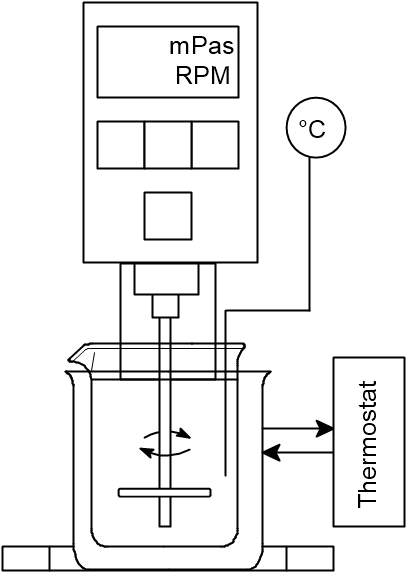
\includegraphics[width=0.25\textwidth]{img/viskosimeter}
%	\caption{Viskositätsmessung mit digitalem \textsc{Brookfield}-\linebreak Rotationsviskosimeter}
%	\label{fig: viskosimeter}
%\end{wrapfigure}
%\FloatBarrier
%%Ende

\begin{figure}[h!]
	\centering
	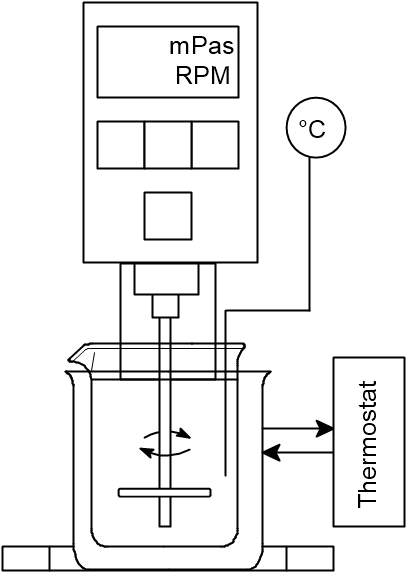
\includegraphics[width=0.25\textwidth]{img/viskosimeter}
	\caption{Viskositätsmessung mit digitalem \textsc{Brookfield}-\linebreak Rotationsviskosimeter}
	\label{fig: viskosimeter}
\end{figure}
\FloatBarrier
%Ende

Die Messung mittels digitalem \textsc{Brookfield}-Viskosimeter ist vergleichsweise einfach. Benötigt werden hierfür das Viskosimeter in einer Halterung, ein Becherglas, ein Temperaturmessgerät und eine herstellerspezifische Spindel. Soll die Viskosität bei bestimmten Temperaturen, abweichend der Labortemperatur bestimmt werden, ist zusätzlich ein thermostatisches Flüssigkeitsbad nötig (vgl. Abb. \ref{fig: viskosimeter}). Die Messung lässt sich nach dem Aufbau über das Bedienfeld starten in dem Spindel und Drehzahl eingegeben werden. Sobald die Messung startet beginnt sich die Spindel zu drehen.\\
Das Messprinzip eines solchen \textsc{Brookfield}-Viskosimeters basiert auf der Messung der Winkelabweichung, auch Torsion genannt, zwischen der im Viskosimeter verbauten Welle und einer zweiten darunter angeordneten Spindel-Welle mit fest definierten geometrischen Körper. Beide Wellen drehen sich dabei mit der selben Drehzahl  und sind über eine Federeinheit verbunden. Bei Digital-Viskosimetern wird der Messwert der sich dann durch die Winkelabweichung ergibt direkt über ein Display angezeigt.\linebreak
Entscheidend für die Messung der Viskosität ist bei dieser Messmethode die Auswahl des bereits erwähnten Becherglases, sowie der Spindel und der Drehzahl. Spindel und Drehzahl werden dabei unter Einbezug des Viskositätbereiches der Probe nach der gewünschten Präzision und dem Geschwindigkeitgefälle ausgewählt. \cite{DINDeutschesInstitutfurNormunge.V..September2018} 
Durch Tabellen des Herstellers, welche sowohl Spindel als auch Viskositätsbereich in Abhängigkeit von Drehzahl und Gerätekonstanten berechnen lassen, werden diese Entscheidungen vereinfacht. \cite{brookfield_31.01.2022} 

\subsubsection{Erwärmungsverhalten}
\subsubsection{Verdünnungsverhalten}
\subsubsection{Pumpversuche}

\subsection{Recherchearbeit: Literaturarbeit, Fachgespräche und Angebotsanfragen}
\todo[inline]{Vielleicht eher später schreiben ?}

\subsection{Gefährdungsbeurteilung (HAZOP-Verfahren)}
%Nur für die entschiedene Variante

\subsection{Computerunterstützes Zeichnen von Plänen mit AutoCAD}




